\documentclass[aspectratio=169,sans]{beamer}

% =====================
% Packages
% =====================
\usepackage[utf8]{inputenc}
\usepackage[T1]{fontenc}
\usepackage{lmodern}
\usepackage{microtype}
\usepackage{graphicx}
\usepackage{amsmath,amssymb}
\usepackage{booktabs}
\usepackage{pgfplots}
\pgfplotsset{compat=1.18}

% =====================
% Global look
% =====================
\setbeamertemplate{navigation symbols}{}
\setbeamertemplate{headline}{}

% Clean, restrained palette
\definecolor{Ink}{HTML}{1B1F24}
\definecolor{Accent}{HTML}{1F4E79}
\definecolor{Muted}{HTML}{6B7280}
\definecolor{Grid}{HTML}{E5E7EB}
\definecolor{Paper}{HTML}{FFFFFF}

\setbeamercolor{background canvas}{bg=Paper}
\setbeamercolor{normal text}{fg=Ink}
\setbeamercolor{structure}{fg=Accent}
\setbeamercolor{frametitle}{fg=Ink,bg=Paper}
\setbeamercolor{title}{fg=Ink}
\setbeamercolor{subtitle}{fg=Muted}
\setbeamercolor{author}{fg=Ink}
\setbeamercolor{institute}{fg=Muted}
\setbeamercolor{date}{fg=Muted}
\setbeamercolor{footline}{fg=Muted,bg=Paper}
\setbeamercolor{block title}{fg=Paper,bg=Accent}
\setbeamercolor{block body}{fg=Ink,bg=Grid!35}
\setbeamercolor{itemize item}{fg=Accent}
\setbeamercolor{itemize subitem}{fg=Muted}

\usefonttheme{professionalfonts}
\setbeamerfont{title}{size=\LARGE,series=\bfseries}
\setbeamerfont{subtitle}{size=\normalsize,series=\mdseries}
\setbeamerfont{frametitle}{size=\large,series=\bfseries}
\setbeamerfont{footline}{size=\scriptsize}
\setbeamerfont{block title}{series=\bfseries}

% =====================
% Frame title
% =====================
\setbeamertemplate{frametitle}{%
  \vspace{0.35cm}
  {\usebeamerfont{frametitle}\insertframetitle}
  \ifx\insertframesubtitle\empty\else
    \par{\small\color{Muted}\insertframesubtitle}
  \fi
  \par\vspace{0.15cm}
  {\color{Grid}\hrule height 0.6pt}
  \vspace{0.15cm}
}

% =====================
% Footline
% =====================
\setbeamertemplate{footline}{%
  \begin{beamercolorbox}[wd=\paperwidth,ht=0.42cm,dp=0.15cm,leftskip=0.35cm,rightskip=0.35cm]{footline}
    \insertshorttitle\hfill\insertframenumber/\inserttotalframenumber
  \end{beamercolorbox}%
}

% =====================
% Itemize / blocks
% =====================
\setbeamertemplate{itemize item}{$\bullet$}
\setbeamertemplate{itemize subitem}{$\circ$}
\setbeamertemplate{blocks}[rounded][shadow=false]

% =====================
% Title page
% =====================
\setbeamertemplate{title page}{%
  \vspace*{1.2cm}
  {\color{Accent}\rule{0.22\paperwidth}{1.2pt}}\par
  \vspace{0.65cm}
  {\usebeamerfont{title}\inserttitle\par}
  \vspace{0.15cm}
  {\usebeamerfont{subtitle}\insertsubtitle\par}
  \vspace{0.55cm}
  {\usebeamerfont{author}\insertauthor\par}
  \vspace{0.08cm}
  {\usebeamerfont{institute}\insertinstitute\par}
  \vspace{0.25cm}
  {\usebeamerfont{date}\insertdate\par}
  \vfill
  {\color{Grid}\rule{0.55\paperwidth}{0.6pt}}\par
  \vspace{0.25cm}
  {\small\color{Muted}Physics seminar template}
}

% =====================
% Metadata
% =====================
\title[Optics Report]{Measurement of Optical Refraction Indices}
\subtitle{Progress Report}
\author[Your Name]{Your Name Here}
\institute[Physics Department]{Department of Physics \and University of Example}
\date{\today}

% =====================
% Document
% =====================
\begin{document}

\begin{frame}[plain]
  \titlepage
\end{frame}

\begin{frame}{Outline}
  \tableofcontents[hideallsubsections]
\end{frame}

\section{Motivation}
\begin{frame}{Why this experiment?}
  \begin{itemize}
    \item Refraction remains a clean test of wave propagation in dielectrics.
    \item The slope of the linear relation encodes the refractive index ratio.
    \item The goal is not decoration; the goal is traceable evidence.
  \end{itemize}

  \begin{block}{Core idea}
    A good physics slide should let the audience read the result in one glance.
  \end{block}
\end{frame}

\section{Model}
\begin{frame}{Snell--Descartes law}
  \begin{equation*}
    n_1\sin\theta_1 = n_2\sin\theta_2.
  \end{equation*}

  \vspace{0.2cm}
  When the first medium is fixed, the measured slope gives a direct estimate of the refractive index ratio.
\end{frame}

\section{Results}
\begin{frame}{Experimental verification}
  \begin{center}
  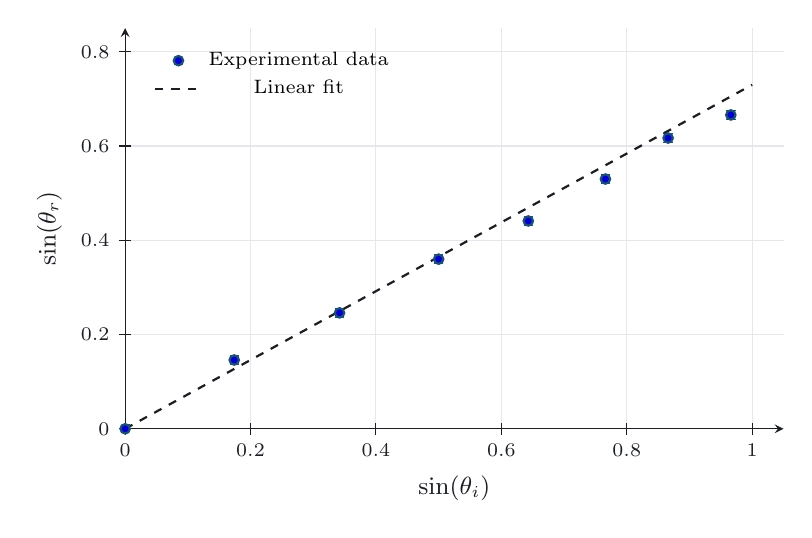
\begin{tikzpicture}
    \begin{axis}[
      width=0.82\textwidth,
      height=0.55\textwidth,
      xlabel={$\sin(\theta_i)$},
      ylabel={$\sin(\theta_r)$},
      xmin=0, xmax=1.05,
      ymin=0, ymax=0.85,
      axis lines=left,
      grid=major,
      major grid style={Grid, thin},
      axis line style={Ink, thin},
      tick style={Ink, thin},
      label style={font=\small, color=Ink},
      tick label style={font=\scriptsize, color=Ink},
      legend style={font=\scriptsize, draw=none, fill=none},
      legend pos=north west,
      mark size=1.7pt,
      every axis plot/.append style={thick},
    ]
      \addplot+[
        only marks,
        mark=*,
        color=Accent,
        error bars/.cd,
          y dir=both,
          y explicit,
          error bar style={Accent, thin},
      ] coordinates {
        (0.000,0.000) +- (0,0.010)
        (0.174,0.146) +- (0,0.010)
        (0.342,0.246) +- (0,0.010)
        (0.500,0.360) +- (0,0.010)
        (0.643,0.441) +- (0,0.010)
        (0.766,0.530) +- (0,0.010)
        (0.866,0.617) +- (0,0.010)
        (0.966,0.666) +- (0,0.010)
      };
      \addlegendentry{Experimental data}

      \addplot[domain=0:1, samples=2, color=Ink, dashed] {0.73*x};
      \addlegendentry{Linear fit}
    \end{axis}
  \end{tikzpicture}
  \end{center}
\end{frame}

\section{Conclusion}
\begin{frame}{Conclusion}
  \begin{itemize}
    \item The data are consistent with a linear refraction model.
    \item The presentation style stays deliberately restrained.
    \item The slide should frame the physics, not compete with it.
  \end{itemize}

  \begin{center}
    \vspace{0.4cm}
    {\large\color{Accent}Questions?}
  \end{center}
\end{frame}

\end{document}
